\documentclass[handout]{mcs}

\begin{document}

\renewcommand{\reading}{
\begin{itemize}
\item
  Chapter~\bref{sec:coloring}--\bref{trees-sec}.\ \emph{Simple
    Graphs: Coloring, Connectedness}

\item Chapter~\bref{chap:asymptotics}
  through~\bref{sec:closed_products}.\ \emph{Sums \& Series}
  (omit~\bref{doublesum_sec})
\end{itemize}}

\problemset{7}

\begin{staffnotes}
\textbf{Potential Topics}: Asymptotics, Counting with Bijections,
Counting Repetitions, Binomial Thm, Pigeonholes Inclusion-Exclusion,
Intro to Discrete Probability, Conditional Probability, Independence

\textbf{TODO} add covered lectures
\end{staffnotes}

%%%%%%%%%%%%%%%%%%%%%%%%%%%%%%%%%%%%%%%%%%%%%%%%%%%%%%%%%%%%%%%%%%%%%
% Problems start here
%%%%%%%%%%%%%%%%%%%%%%%%%%%%%%%%%%%%%%%%%%%%%%%%%%%%%%%%%%%%%%%%%%%%%

\begin{staffnotes}
Most of the ones in the list are pretty good, but we can change the
$2^{n/2}$ one to $4^n$ and $2^n$, and the $\sin$ to a $\cos$.
\end{staffnotes}

\pinput{PS_asymptotics_table}

\pinput{PS_5_card_poker}

%%fa14 pset 10 problem 3
\instatements{\vspace{0.5in}}
\begin{problem}
We're covering probability in 6.042 lecture one day, and you volunteer
for one of Professor Leighton's demonstrations. He shows you a coin
and says he'll bet you \$1 that the coin will come up heads. Now,
you've been to lecture before and therefore suspect the coin is
biased, such that the probability of a flip coming up heads, $\pr{H}$,
is $p$ for $1/2 < p \leq 1$.

You call him out on this, and Professor Leighton offers you a
deal. He'll allow you to come up with an algorithm using the biased
coin to \textit{simulate} a fair coin, such that the probability you
win and he loses, $\pr{W}$, is equal to the probability that he wins
and you lose, $\pr{L}$. You come up with the following algorithm:

\begin{enumerate}
\item Flip the coin twice.
\item Based on the results:
        \begin{itemize}
        \item $TH \implies$ you win [$W$], and the game terminates.
        \item $HT \implies$ Professor Leighton wins [$L$], and the game terminates.
        \item $(HH \lor TT) \implies$ discard the result and flip again.
        \end{itemize}
\item If at the end of $N$ rounds nobody has won, declare a tie.
\end{enumerate}
As an example, for $N=3$, an outcome of $HT$ would mean the game ends
early and you lose, $HHTH$ would mean the game ends early and you win,
and $HHTTTT$ would mean you play the full $N$ rounds and result in a
tie.

\bparts

\ppart
Assume the flips are mutually independent. Show that $\pr{W} = \pr{L}$.

\begin{solution}
The probability of you winning is equal to the probability that you
win in the first round, plus the probability that nobody won in the
first round times the probability that you win in the second round,
plus the probability that nobody won in the first two round times the
probability that you win in the third round, etc. The same goes for
Professor Leighton. Hence:
\begin{align*}
\pr{W} &= \pr{TH} + \pr{HH \lor TT}\pr{TH} + \pr{HH \lor TT}^2\pr{TH} + \ldots \\
& = \pr{TH} \cdot \sum_{i=0}^N \pr{HH \lor TT}^i \\
& = \pr{HT} \cdot \sum_{i=0}^N \pr{HH \lor TT}^i\\
& = \pr{L}
\end{align*}
The middle step is possible because $\pr{TH} = (1-p)p = p(1-p) = \pr{HT}$.

\end{solution}

\ppart
Show that, if $p<1$, the probability of a tie goes to 0 as $N$ goes to infinity.

\begin{solution}

The probability of a tie is just the probability that nobody won all $N$ rounds, namely:
\[
\pr{tie} = (\pr{HH \lor TT})^N = (\pr{HH} + \pr{TT})^N = (p^2 + (1-p)^2)^N
\]
So the limit as $N$ goes to infinity is 0, given that $p$ and
therefore $p^2 + (1-p)^2$ are $< 1$.

\end{solution}

\eparts

\end{problem}


\pinput{PS_monochromatic_rectangle}

\begin{staffnotes}
fa14 pset 10 problem 2, we could change to 401 integers less than 500,
quotient is a power of 5
\end{staffnotes}

\begin{problem}
In lecture we discussed the Birthday Paradox. Namely, we found that in
a group of $m$ people with $N$ possible birthdays, if $m \ll N$, then:
\[
\pr{\text{all $m$ birthdays are different}} \sim e^{-\frac{m(m-1)}{2N}}
\]
To find the number of people, $m$, necessary for a half chance of a
match, we set the probability to $1/2$ to get:
\[
m \sim \sqrt{(2\ln2)N} \approx 1.18\sqrt{N}
\]

For $N = 365$ days we found $m$ to be 23.

We could also run a different experiment. As we put on the board the
birthdays of the people surveyed, we could ask the class if anyone has
the same birthday. In this case, before we reached a match amongst the
surveyed people, we would already have found other people in the rest
of the class who have the same birthday as someone already
surveyed. Let's investigate why this is.

\bparts

\ppart Consider a group of $m$ people with $N$ possible birthdays
amongst a larger class of $k$ people, such that $m \leq k$. Define
$\pr{A}$ to be the probability that $m$ people all have different
birthdays \textit{and} none of the other $k-m$ people have the same
birthday as one of the $m$.

Show that, if $m \ll N$, then $\pr{A} \sim
e^{\frac{m(m-2k)}{2N}}$. (Notice that the probability of no match is
$e^{-\frac{m^2}{2N}}$ when $k$ is $m$, and it gets smaller as $k$ gets
larger.)

\hspace{0.5in} \textit{Hints:} For $m \ll N$: $\frac{N!}{(N-m)!N^m}
\sim e^{-\frac{m^2}{2N}}$, and $(1-\frac{m}{N}) \sim
e^{-\frac{m}{N}}$.

\begin{solution}

We know:
\[
\pr{A} = \frac{N(N-1)\ldots(N-m+1)\cdot(N-m)^{k-m}}{N^k}
\]

since there are $N$ choices for the first birthday, $N-1$ choices for
the second birthday, etc., for the first $m$ birthdays, and $N-m$
choices for each of the remaining $k-m$ birthdays. There are total
$N^k$ possible combinations of birthdays within the class.

\begin{align*}
\pr{A} &= \frac{N(N-1)\ldots(N-m+1)\cdot(N-m)^{k-m}}{N^k} \\
&= \frac{N!}{(N-m)!}\left(\frac{(N-m)^{k-m}}{N^k}\right) \\
&= \frac{N!}{(N-m)!N^m}\left(\frac{N-m}{N}\right)^{k-m} \\
&= \frac{N!}{(N-m)!N^m}\left(1-\frac{m}{N}\right)^{k-m} \\
&\sim e^{-\frac{m^2}{2N}} \cdot e^{-\frac{m}{N}(k-m)} & \text{(by the Hint)} \\
& = e^{\frac{m(m-2k)}{2N}}
\end{align*}
\end{solution}

\ppart Find the approximate number of people in the group, $m$,
necessary for a half chance of a match (your answer will be in the
form of a quadratic). Then simplify your answer to show that, as $k$
gets large (such that $\sqrt{N} \ll k$), then $m \sim
\frac{N\ln2}{k}$.

\hint $x \ll 1$: $\sqrt{1-x} \sim (1-\frac{x}{2})$.

\begin{solution}

Setting $\pr{A} = 1/2$, we get a solution for $m$:

\begin{align*}
1/2 &= e^{\frac{m(m-2k)}{2N}} \\
-2N\ln2 &= m^2 -2km  \\
0 &= m^2-2km + (2N\ln2) \\
m &= \frac{2k \pm \sqrt{(2k)^2 - 4(2N\ln2)}}{2}
\end{align*}

Simplifying the solution under the assumption of large $k$, we find:
\begin{align*}
m &= \frac{2k - \sqrt{4k^2 - 8N\ln2}}{2} & \text{(taking the lower positive root)} \\
&= k - k\sqrt{1 - \frac{2N\ln2}{k^2}} \\
&\sim k  - k \left(1-\frac{2N\ln2}{2k^2}\right) & \text{(by the Hint)} \\
&= \frac{N\ln2}{k}
\end{align*}

\end{solution}

\eparts

\end{problem}


\pinput{PS_path_counting}


\pinput{PS_four_door_random_or_not} %extends the monty hall problem to
                                    %4 door

\begin{staffnotes}
F07.Ps10.Prob4, F08.ps11.prob4
\end{staffnotes}

\begin{problem}
Independently flip three fair coins (with ``fair'' meaning ``equally likely to come
up with a head or a tail").
\begin{itemize}
\item Let $H_i$ be the indicator variable for a head occurring on the $i$th flip, for $i=1,2,3$,
\item $C$ be the random variable for the number of heads flipped, $H_1+H_2+H_3$,
\item $M$ to be the indicator variable for the event that all three coins match, $[H_1=H_2=H_3]$,
\item and $S$ be the indicator variable for the event that an odd number of heads are flipped, $[C \equiv 1 \mod 2]$.
\end{itemize}

\bparts

\ppart\label{depC} Show that none of these six variables is independent of $C$.

\hint Consider the case when $C=3$.

\begin{solution}
If $C=3$, then the values of all the other variables are determined, namely $H_1=H_2=H_3=M=S=1$.  

Therefore, for all six variables $V$, $\prcond{V=1}{C=3} = 1$, but $\pr{V=1}\neq 1$. So
\[
\prcond{V=1}{C=3} \neq \pr{V=1}
\]
for all six variables, $V$, which shows that none of them is independent of $C$.
\end{solution}

\ppart Show that $M$ and $S$ are pairwise independent.

\begin{solution}
To see that $M$ and $S$ are pairwise independent, we check each of the cases.
\begin{align*}
\pr{S=0 \text{ and } M=0} & = \pr{HHT,HTH,THH}\\
    & = \frac{3}{8} = \frac{1}{2} \cdot \frac{3}{4} =\pr{S=0} \cdot \pr{M = 0}\\
\pr{S=0 \text{ and } M=1} & = \pr{TTT}\\
    & = \frac{1}{8} = \frac{1}{2} \cdot \frac{1}{4} =\pr{S=0} \cdot \pr{M = 1}\\
\pr{S=1 \text{ and } M=0} & = \pr{TTH,THT,HTT}\\
    & = \frac{3}{8} = \frac{1}{2} \cdot \frac{3}{4} =\pr{S = 1} \cdot \pr{M = 0}\\
\pr{S=1 \text{ and } M=1} & = \pr{HHH}\\
    & = \frac{1}{8} = \frac{1}{2} \cdot \frac{1}{4} =\pr{S = 1} \cdot \pr{M = 1}.
\end{align*}
\end{solution}

\ppart\label{H123S} Show that $H_1,H_2,H_3$, and $S$ are 3-wise
independent, but not mutually independent.

\begin{solution}
Since $H_1,H_2,H_3$ determine all the other variables, then by
the same kind of argument used in part~\eqref{depC}, no set of four or
more variables including these three can be mutually independent.

The variables $H_1,H_2,H_3$ are 3-wise independent by definition of
``flipping independently.''  Now consider the three variables $H_1,H_2,S$.
\begin{align*}
\lefteqn{\pr{S=a \text{ and } H_1=b \text{ and } H_2=c}}\\
  & = \pr{(b+c+H_3 \equiv a \mod 2) \text{ and } H_1=b \text{ and } H_2=c}
      & ([S=a] ::= [H_1+H_2+H_3 \equiv a \mod 2])\\
  & = \pr{H_3 = rem(a-b-c,2) \text{ and } H_1=b \text{ and }
  H_2=c}\\
  & = \pr{H_3 = rem(a-b-c,2)}\cdot \pr{H_1=b} \cdot \pr{H_2=c} &
  \text{(independence of the flips)} \\
& = (1/2)^3 \\
& = \pr{S=a} \cdot \pr{H_1=b} \cdot \pr{H_2=c} &
  \text{(since $\pr{S=a}=1/2$)}.
\end{align*}
Likewise for $S$ and any other two $H_i$'s.  So $H_1,H_2,H_3$, and $S$ are
3-wise independent because any three of them are mutually independent.
\end{solution}

\iffalse
\ppart Show that the five variables other than $C$ are pairwise independent.

\begin{solution}

Part~\eqref{H123S} already shows that any two of $H_1,H_2,H_3,$ and $S$
are pairwise independent, so we need only verify that $H_i$ and $M$ are
pairwise independent and that $S$ and $M$ are pairwise independent.

To see that $H_i$ and $M$ are pairwise independent, we just check the cases where $i = 1$ and $H_1 =1$. The other cases are symmetric.
\begin{align*}
\pr{H_1=1 \text{ and } M=0} & = \pr{HTT, HHT, HTH}\\
    & = \frac{3}{8} = \frac{1}{2} \cdot \frac{3}{4} =\pr{H_1 = 1} \cdot \pr{M = 0}\\
\pr{H_1=1 \text{ and } M=1} & = \pr{HHH}\\
    & = \frac{1}{8} = \frac{1}{2} \cdot \frac{1}{4} =\pr{H_1 = 1} \cdot \pr{M = 1}.
\end{align*}

To see that $S$ and $M$ are pairwise independent, we check each of the cases.
\begin{align*}
\pr{S=0 \text{ and } M=0} & = \pr{HHT,HTH,THH}\\
    & = \frac{3}{8} = \frac{1}{2} \cdot \frac{3}{4} =\pr{S=0} \cdot \pr{M = 0}\\
\pr{S=0 \text{ and } M=1} & = \pr{TTT}\\
    & = \frac{1}{8} = \frac{1}{2} \cdot \frac{1}{4} =\pr{S=0} \cdot \pr{M = 1}\\
\pr{S=1 \text{ and } M=0} & = \pr{TTH,THT,HTT}\\
    & = \frac{3}{8} = \frac{1}{2} \cdot \frac{3}{4} =\pr{S = 1} \cdot \pr{M = 0}\\
\pr{S=1 \text{ and } M=1} & = \pr{HHH}\\
    & = \frac{1}{8} = \frac{1}{2} \cdot \frac{1}{4} =\pr{S = 1} \cdot \pr{M = 1}.
\end{align*}

\end{solution}

\ppart Show that $H_1,S$ and $M$  are not mutually independent.

\begin{solution}
If $H_1=1$ and $S=0$, then $M=0$.  Hence,

\begin{align*}
\pr{H_1=1 \text{ and } S=0 \text{ and } M=0} & = \pr{H_1=1 \text{ and } S=0}\\
    & = \pr{H_1=1}\cdot \pr{S=0}  & \text{(part~\eqref{H123S})}\\
    & = \frac{1}{2} \cdot  \frac{1}{2}\\
    & \textcolor{red}{\neq} \frac{1}{2} \cdot  \frac{1}{2} \cdot \frac{3}{4}\\
    & = \pr{H_1=1}\cdot \pr{S=0} \cdot \pr{M=0}.
\end{align*}
\end{solution}

\ppart Show that no set of three variables including both $M$ and $H_i$
for any $i\in \set{1,2,3}$ is 3-wise independent.

\begin{solution}

We've seen that $H_1,S$, and $M$ are not mutually independent.
  The same reasoning can be applied when substituting $H_2$ or $H_3$ for
  $H_1$.  We've also seen that none of the variables is independent of
  $C$, so $C$ cannot be one of the three variables in the set and still
  have the set be 3-wise independent.

  That leaves sets of the form $\set{M, H_i, H_j}$, $i$ and $j$ not equal
  and between 1 and 3.  If $H_i = H_j = M = 1$, then all coins are heads.

\begin{align*}
\pr{H_i=1 \text{ and } H_j = 1 \text{ and } M=1} & = \pr{H_1=1 \text{ and } H_2 = 1 \text{ and } H_3 =1}\\
    & = \pr{H_1=1}\cdot \pr{H_2 = 1} \cdot \pr{H_3 = 1}  & \text{(indep. of $H_i$'s)}\\
    & = \frac{1}{2} \cdot  \frac{1}{2} \cdot \frac{1}{2}\\
    & \textcolor{red}{\neq} \frac{1}{2} \cdot  \frac{1}{2} \cdot \frac{1}{4}\\
    & = \pr{H_i=1}\cdot \pr{H_j=1} \cdot \pr{M=1}.
\end{align*}
\end{solution}
\fi

\eparts
\end{problem}


\begin{problem}
\begin{staffnotes}
F98 Basic probability, F01.ps10.prob1
\end{staffnotes}

Compute the probabilities of the following three events and determine
which one is most likely.  Assume that the dice are fair, 6-sided, and
mutually independent.

\begin{problemparts}
\problempart Rolling at least one 6 when six dice are rolled.

\begin{solution}
The probability of rolling a 6 on a particular die is $1/6$.  The
probability of not rolling a 6 on a particular die is $5/6$, since
this is the complementary event.  The probability of not rolling a 6
on any of six dice is $(5/6)^6$, since the numbers rolled are mutually
independent.  The probability of rolling a 6 on some die is therefore
\[
1 - (\frac{5}{6})^6 = 0.665\ldots.
\]
\end{solution}

\problempart Rolling at least two 6's when twelve dice are rolled.

\begin{solution}
The probability of rolling two or more 6's is 1 minus the probability
of rolling zero or one 6's.  The probability of rolling zero 6's is
$(5/6)^{12}$, arguing as before.  The probablity of rolling exactly
one 6 is
\[
12 \cdot \frac{1}{6} \cdot \left(\frac{5}{6}\right)^{11}
\]
since there are 12 ways to choose the die that comes up 6, the
probability of this die coming up 6 is $\cfrac{1}{6}$, and the
probability of the remaining dice all coming up in the range 1 to 5 is
$(5/6)^{11}$.  Overall, the probability of rolling two or more sixes
is therefore
\begin{eqnarray*}
1 - \left(\frac{5}{6}\right)^{12} -
        12 \cdot \frac{1}{6} \cdot \left(\frac{5}{6}\right)^{11}
                & = &   0.618\ldots.
\end{eqnarray*}

\end{solution}

\problempart Rolling at least three 6's when eighteen dice are rolled.

\begin{solution}
Arguing as before, the probability of rolling at least three 6's is

\begin{eqnarray*}
1       - \left(\frac{5}{6}\right)^{18}
        - 18 \cdot \frac{1}{6} \cdot \left(\frac{5}{6}\right)^{17}
        - \binom{18}{2} \cdot \left(\frac{1}{6}\right)^2 \cdot
                \left(\frac{5}{6}\right)^{16}
        & = &   0.597\ldots.
\end{eqnarray*}
\end{solution}

\end{problemparts}

\begin{solution}
The first event is most likely.
\end{solution}
\end{problem}

\begin{staffnotes}
F00 tournament probabilities, F01.ps10,prob3
\end{staffnotes}

\begin{problem}
A tennis tournament has 8 players. The players are assigned randomly
to positions in the first round of a tournament ladder (see
Figure~\ref{tennis}).

\begin{figure}%[htbp]
%\centerline{\psfig{figure=/a/class/6.042/fall00/handouts/fig/H64-tennis.eps,height=4in}}
\centerline{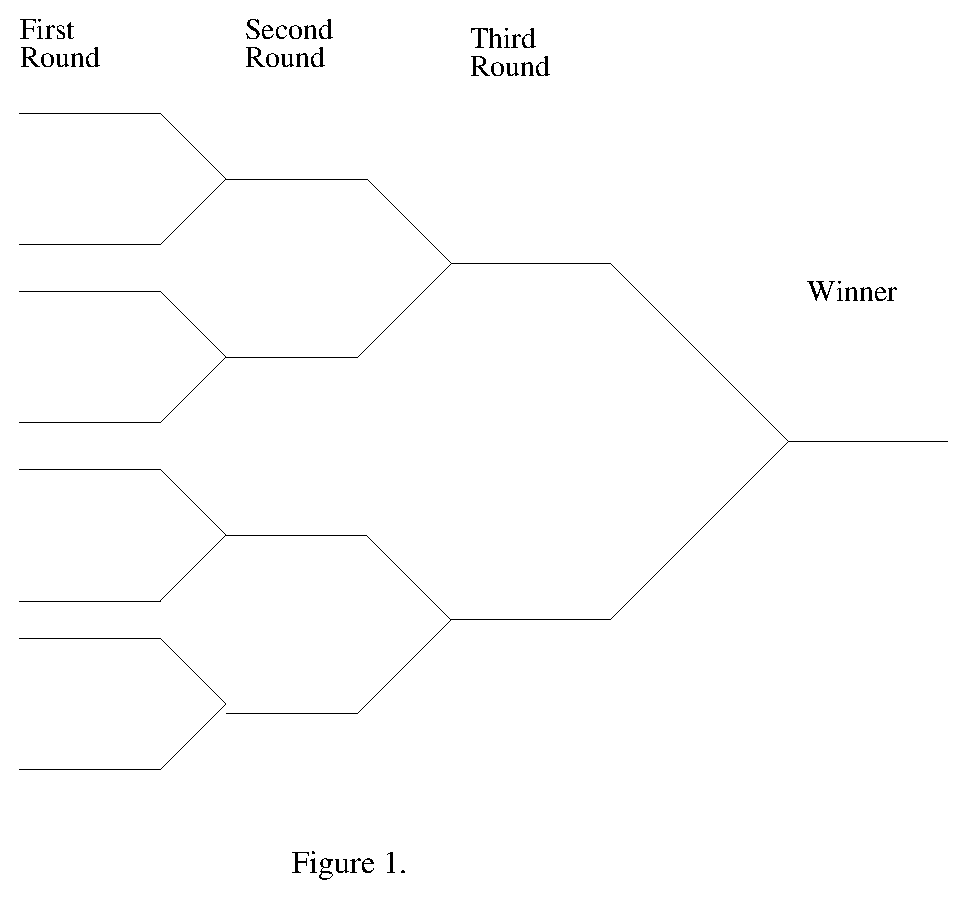
\includegraphics[height=4in]{H64-tennis}}
\caption{Tournament Tree}
\label{tennis}
\end{figure}

\bparts

\ppart
Suppose the best player always defeats everybody else, and
the second-best player always defeats everybody but the best. What
is the chance that the second-best player makes it to the final round?

\begin{solution}
In order to make it to the final round, the
second-best player has to meet
the winner in the final round and not earlier.
That happens if and only if the best
player and the second-best player start out in different brackets of
four; in other words, if the best player starts in position 1-4 of the
first round, then the second-best must start in positions 5-8, and
vice versa.

Here are two ways to determine the probability.  The first way counts
complete assignments: there are 8 ways to place the best player in the
first round, then 4 ways to place the second-best, then $6!$ ways to
place the remaining players.  Divide by the size of the sample space
($8!$, the total number of ways to assign all eight players with no
constraints) to get $4/7$.

The second way treats the second player's position as a random selection.
The best player can be placed anywhere.  Given the best player's position,
the second-best player will meet the first player in the final round
only if he is placed in 4 of the remaining 7 positions---not 4 out of 8,
because the best player is already occupying one (this is a common error
-- the positions of the players can't be treated like independent coin
flips or dice rolls, because no two players can occupy the same
position.)!  Since all placements are equally likely, there is a $4/7$
chance of this happening.
\end{solution}

\ppart Suppose the 8 tennis players are equally good, i.e.,
for any two players A and B,
\[
\prob{A \mbox{ wins}}=\prob{B \mbox{ wins}}= 1/2,
\]
and the twins Tom and Mot are amongst the 8 players.  What is the chance
that Tom and Mot ever meet in a match during the tournament?

\begin{solution}

The probability that Tom and Mot will meet in the first round is $1/7$
(Tom can be placed anywhere, but given Tom's position, Mot has only 1
choice in 7).

Tom and Mot will meet in the second round if and only if both win
their first-round matches (with probability $1/2 \cdot 1/2$) and both
are in different groups of two but the same group of four (probability
$2/7$).

Tom and Mot will meet in the third round if and only if both win two
matches (with probability $1/2^2 \cdot 1/2^2$) and both are in different
groups of four (probability $4/7$).

Since these events are disjoint, the probability that Tom and Mot meet in
any round is just the sum:
\[
\frac{1}{7} + \frac{1}{2} \cdot \frac{1}{2} \cdot \frac{2}{7}
+ \frac{1}{4} \cdot \frac{1}{4} \cdot \frac{4}{7} = \frac{1}{4}
\]
\end{solution}

\eparts

\end{problem}

\end{document}
